% Chapter 5

\chapter{Implementation}
\label{Chapter5}
\lhead{Chapter 5. \emph{Implementation}}
\sloppy

\section{Repository and Source Availability}
The IronClaw implementation is maintained as a Rust workspace. The project is
hosted at:
\begin{center}
\url{https://github.com/suryavirkapur/ironclaw}
\end{center}

The local repository is organized around a host daemon, a guest runtime, shared
protocol and transport crates, tool implementations, security helpers, memory
support, channel integrations, configuration files, Firecracker build assets,
and smoke-test scripts. This structure keeps the host-facing control plane
separate from the guest execution plane.

\section{Workspace Organization}
The core workspace directories are:
\begin{itemize}
    \item \texttt{crates/ironclawd}: the host daemon, API server, agent loop,
    sandbox manager, provider integration, channel integration, and dispatch
    logic.
    \item \texttt{crates/irowclaw}: the guest runtime that executes inside the
    sandbox boundary and handles tool execution requests.
    \item \texttt{crates/common}: shared configuration structs, protobuf
    bindings, Firecracker abstractions, codec, transport traits, and stream
    transport.
    \item \texttt{crates/tools}: concrete tool implementations such as
    workspace-bounded file read/write, restricted shell execution, and browser
    automation.
    \item \texttt{crates/memory}: SQLite-backed memory, markdown indexing,
    hybrid retrieval, redaction, and pinned memory operations.
    \item \texttt{crates/security}: authentication, pairing, and rate-limiting
    components used by external control surfaces.
    \item \texttt{crates/channels}: messaging channel integrations.
    \item \texttt{configs/}: host and guest TOML configuration files.
    \item \texttt{scripts/}: root filesystem build scripts and smoke tests for
    local, container, websocket, and Firecracker paths.
\end{itemize}

\section{Host Configuration}
The host daemon is configured through \texttt{configs/ironclawd.toml}. The file
selects the execution mode, sandbox runtime, guest protocol, API bind address,
LLM provider endpoint, Firecracker assets, container runtime settings, daemon
log files, and channel integration settings. A representative excerpt is:
\begin{verbatim}
execution_mode = "auto"
sandbox_runtime = "container"
guest_protocol = "proto"
idle_timeout_minutes = 5
log_level = "info"

[server]
bind = "127.0.0.1"
port = 9938

[llm]
model = "glm-5.2"
base_url = "https://opencode.ai/zen/go/v1"
api = "chat_completions"

[firecracker]
enabled = false
kernel_path = "kernels/firecracker/vmlinux-6.1.155.bin"
rootfs_path = "rootfs/build/guest-rootfs.ext4"
api_socket_dir = "/tmp/ironclaw-fc"
vsock_uds_dir = "/tmp/ironclaw/vsock"
vsock_port = 5000

[container]
engine = "docker"
image = "ironclaw/irowclaw:latest"
network = "bridge"
brain_mount_path = "/mnt/brain"
command = ["irowclaw"]
\end{verbatim}

The configuration maps directly to strongly typed Rust structures in
\texttt{crates/common/src/config.rs}. The host supports multiple execution
modes: \texttt{auto}, \texttt{host\_only}, \texttt{guest\_tools}, and
\texttt{guest\_autonomous}. It also supports multiple sandbox runtime choices:
\texttt{auto}, \texttt{process}, \texttt{container}, and \texttt{microvm}. This
allows the same higher-level agent loop to be evaluated under different
containment strategies.

\section{Guest Configuration}
The guest runtime is configured with \texttt{irowclaw.toml}, normally mounted at
\texttt{/mnt/brain/config/irowclaw.toml}. The default guest configuration keeps
shell access disabled and allows file tools:
\begin{verbatim}
default_agent = "default"
log_level = "info"

[tools]
allow_bash = false
allow_file = true

[browser]
headless = true
timeout_ms = 30000
allowed_domains = []
max_memory_mb = 512
max_cpu_seconds = 20

[indexing]
max_chunk_bytes = 2048
embedding_model = "text-embedding-3-small"
vector_weight = 0.7
keyword_weight = 0.3
embedding_cache_size = 1000

[scheduler]
jobs_path = "/mnt/brain/cron/jobs.toml"
\end{verbatim}

For controlled testing, \texttt{configs/irowclaw.allow-bash.toml} enables the
shell tool and sets \texttt{allowed\_domains = ["*"]}. This is useful for
development and red-team experiments, but the safer default keeps network and
shell authority narrow.

\section{Protocol and Framing}
Host and guest communicate using a protobuf message envelope defined in
\texttt{crates/common/proto/ironclaw.proto}. Each message carries
\texttt{user\_id}, \texttt{session\_id}, \texttt{msg\_id},
\texttt{timestamp\_ms}, and a \texttt{cap\_token}. The payload is a protobuf
\texttt{oneof} that can represent authentication, agent control, user messages,
tool calls, tool responses, file operations, scheduler events, or streaming
deltas.

The current envelope supports:
\begin{itemize}
    \item \texttt{AuthChallenge} and \texttt{AuthAck} for guest authorization;
    \item \texttt{AgentControl} and \texttt{AgentState} for sleep/wake control;
    \item \texttt{UserMessage} for user-originated text;
    \item \texttt{ToolCallRequest} and \texttt{ToolCallResponse} for tool
    execution;
    \item \texttt{FileOpRequest} and \texttt{ToolResult} for bounded file
    operations;
    \item \texttt{JobTrigger} and \texttt{JobStatus} for scheduler integration.
\end{itemize}

The protobuf bytes are length-prefixed by \texttt{ProtoCodec}. The codec writes
a four-byte big-endian frame length followed by the encoded protobuf payload.
This same codec is used over in-memory local transport, child-process standard
I/O, and stream transports such as Firecracker vsock. Keeping framing separate
from the transport lets IronClaw test protocol behavior without requiring a
microVM for every unit test.

\begin{figure}[htbp]
    \centering
    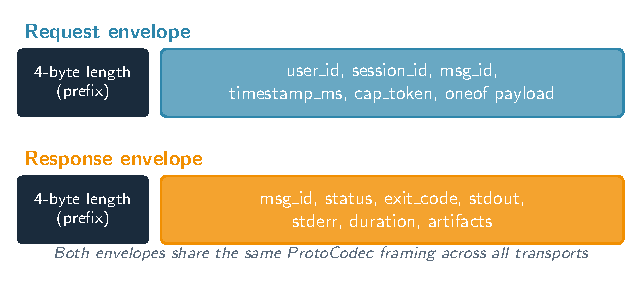
\includegraphics[width=0.95\linewidth]{Figures/fig_protocol_envelope.pdf}
    \caption{Host/guest protobuf message envelope used for all execution requests and responses.}
    \label{fig:protocol_envelope}
\end{figure}

\fref{fig:protocol_envelope} shows the request and response envelope structure.
\section{Authentication and Capability Handshake}
Prior to the runtime execution, the guest runtime will wait for an AuthChallenge
message from the host. The host then sends a capability token to the guest,
containing details regarding the authorization given to the runtime. Additionally,
the host also supplies the guest with a list of allowed tools and the preferred
mode of operation for the guest. After receiving this capability token, the guest
runtime will send an AuthAck message to confirm receipt of the token. Finally,
the guest will utilize the tool allow-list provided by the host to filter out
unauthorized tools from its ToolRegistry.

This capability-based handshaking method offers several important advantages to
this system: It gives the host one place to define session authority; It allows
for various methods to initiate the guest (different runtimes (e.g., process,
container, Firecracker)); It enables the guest to create all possible tools when
compiling its image prior to deployment and also gives the host complete control
of what tools are made accessible to the guest during each individual session.

\section{Sandbox Runtime Implementations}
\texttt{fire-cracker.rs} provides implementations for three sandbox abstractions:
\begin{itemize}
    \item VmManager: Manages VM Lifecycle (Start/Stop), returns information about
    current state of the vm instance.
    \item GuestRuntime: Contains everything required to manage a sandboxed
    runtime. Returned by VmManager.
    \item Transport: Used to communicate between host and guest.
\end{itemize}

\subsection{Process Runtime}
Two forms of local transport exist for testing and rapid development
environments. Local transports have extremely low overhead relative to launching
a new container or creating a new Firecracker microVM. Local transports however
cannot provide the same degree of isolation offered by containers and
microVM's. For example, if you wanted to test generated code that was supposed
to execute in an untrusted environment, you would likely choose to use a
container or a microVM instead of a local transport.

\subsection{Container Runtime}
IronClawD’s container manager (found in
\texttt{ironclawd/src/sandbox.rs}) uses docker to launch the guest runtime within
a container. Prior to starting the guest runtime, the container manager executes
the following actions:
\begin{itemize}
    \item Sanitizes the container name from user ID.
    \item Places a copy of the user's per-user brain directory into the container.
    \item Configures communication between the host and guest by setting
    environmental variables:
    \begin{itemize}
        \item \texttt{IRONCLAW BRAIN ROOT}: The path representing the brain root
        for the user in the guest. This root contains all files associated with
        memory.
        \item \texttt{IROCLAW\_CONFIG}: The path where the guest can locate its
        configuration file.
    \end{itemize}
\end{itemize}

All communication between the host and container occur via standard input/output
streams utilizing ChildPipeTransport. Any errors produced by the container are
sent directly from the container's standard error output to the host. Since both
the container and processes executing on the shared kernel space of the host
share their kernel space, it is generally accepted as being a less secure
boundary than that defined by microVM.

\subsection{Firecracker Runtime}
The Firecracker Manager (located in \texttt{ironclawd/src/sandbox.rs}) manages
Firecrackers creation and start-up process. Creation involves locating/building
kernels and root filesystems images, brain disk images, API socket and vsock
endpoint images. After creation, a Firecracker process spawns and waits for a
socket connection to an API socket. Once connected, Firecracker can be configured
with multiple API calls.

In addition to spawning a process, configuration for Firecracker's microVM can
be accomplished via specifying boot arguments. Some examples of boot arguments
include:
\begin{itemize}
    \item \texttt{console=ttyS0}: Directs console output to \texttt{/dev/ttyS0}.
    \item \texttt{panic=1}: If a fatal error occurs in the microVM, Firecracker
    immediately panics and exits.
    \item \texttt{pci=off}: Disallows enumeration of PCI devices in the microVM.
    \item \texttt{nomodules}: Disables module loading in the kernel.
    \item \texttt{root=/dev/vda}: Indicates that \texttt{/dev/vda} is mounted at
    root (/).
    \item \texttt{init=/init}: Tells init that it should call itself after
    mounting \texttt{/proc /sys /etc}...
\end{itemize}
Boot arguments are supplied to Firecracker via \texttt{--kernel-bootargs}.

Once InstanceStart has been successfully completed by the Firecracker manager, the host attempts to connect to a vsock unix domain socket (vsock:///unix/path/to/socket). The Firecracker manager had previously established a vsock device with guestCID 3. Once connected, the host issues a CONNECT command to establish a stream. In order for this connection attempt to succeed, the guest must listen on a vsock port (which is identified via a command line argument: \texttt{IRONCLAW\_VSOCK=1}) once it reaches InstanceStart.

Once a successful OK response is received from the guest runtime after sending a CONNECT command, the host wraps the stream in StreamTransport and continues to send/receive commands/envelopes as it would with other runtimes.

\section{Guest Runtime Inner Loop}
The guest runtime performs an initialization process which includes:
\begin{itemize}
    \item reading configuration data from \texttt{config.json}
    \item setting up logging
    \item creating directories for brains
    \item opening a sqlite database
    \item initializing memory schema
    \item create a workspace directory
    \item register the tools
    \item enter the transport loop
\end{itemize}

The default path for brain directories is \texttt{/mnt/brain}. The default path
for the workspace is \texttt{/mnt/brain/workspace}. All file-based tools live in
the Workspace Directory.

The runtime loop uses \texttt{tokio::select!} to allow concurrent handling of
both Host messages and Scheduler events. Additionally, a simple power state is
stored to \texttt{config/agent\_state.toml}. Messages sent by agentcontrol can put
the guest runtime into a sleeping state or wake the guest Runtime out of its
sleeping state. While the runtime is sleeping, user messages that request tool
Invocation will receive an explicit rejection message.

First, local memory commands contained within user messages are processed.
Second, prompts are injected and policies are checked. Based upon the execution
mode chosen (the type of Execution allowed), it will send a notification to the
Host that execution in the guest is prohibited, Request that the Host choose a
tool invocation for planning purposes, or execute autonomously with a simple
planner.

\section{Tool Registry and Tool Implementations}
Tools that exist in the guest register themselves in a \texttt{ToolRegistry}.
Although registration and authorization are now separate; although a tool may be
registered in the registry, it will still be denied Unless the name of the tool
exists in the Host's provided Allow-List.

File-based tools utilize a Rooted Path Resolver. Any absolute path (which includes
Parent-Directories) and Platform Specific Prefixes are not permitted as they
would potentially be used to attempt escapes from the Workspace Root such as
\texttt{../../etc/passwd}.

The Restricted Shell Tool executes commands via \texttt{sh -lc} inside the
Workspace Directory. Obvious High-Risk Substrings (such as \texttt{sudo},
\texttt{curl}, \texttt{wget}, \texttt{ssh}, \texttt{scp}, \texttt{nc},
\texttt{netcat}, \texttt{file://}, \texttt{data:}, and \texttt{javascript:}) are
blocked. Output is capped at 32 KiB and Truncated if necessary. Note: these
Safety Checks do not replace Micro VM Isolation; they are defense in Depth
within the guest.

The Browser Tool Launches a Headless Chromium-Compatible Web-Browser. It supports
Fetch requests and screenshot requests as well as JavaScript Evaluation
Requests. It validates url schemes, blocks URLs starting with \texttt{file:},
\texttt{data:}, and \texttt{javascript:}, requires http(s) scheme, enforces a
list of allowable domains, applies some process Limits and expects a timeout.
Screenshot Results returned are encoded as base64 Strings.

\section{Memory and Scheduler Integration}
The guest runtime creates a sqlite backed memory store and then Uses Hybrid
Retrieval over markdown Chunks. Configuration controls chunk size, Embedding
Model, vector weight, Keyword Weight, and Embedding Cache Size. The memory
commands provide explicit pinned memory insertion, listing and Forgetting.
Secrets are redacted before user-provided memories are stored.

The scheduler reads jobs from \texttt{/mnt/brain/cron/jobs.toml}. Scheduler
triggers are converted into protocol messages so that the same transport path
can be utilized for scheduled work and Interactive Work. A scheduled job can
awaken a sleeping runtime and instead of dumping unbounded Output into the
message stream return a log reference.

\section{Security Checks and Output Sanitization}
A layer of safety has been implemented by the guest prior to executing each tool.
The inputs have been checked for patterns of prompt-injectable attacks and Policy
violations. The outputs have been checked for possible leaks before being
returned. This provides ironclaw multiple gates: Host-side Policy before
dispatch, guest-side Policy before execution, tool-specific restrictions during
execution and outbound sanitization after execution.

\section{Testing and Smoke Scripts}
Testing exists in the Codebase for all of the following: Runtime Configuration;
Vsock Transport; Scheduler Behavior; safety handling; browser behavior; Sandbox
Runtime Behavior; Webhook Handling; Channel Handling; Daemon Lifecycle; core
protocol modules.

Smoke Scripts located under \texttt{scripts/} test major deployment paths:
\begin{enumerate}
    \item \texttt{Smoke-local-guest.sh}: test local guest path;
    \item \texttt{Smoke-firecracker.sh}: test firecracker boot path;
    \item \texttt{Smoke-firecracker-ws.sh}: test Firecracker Websocket Path;
    \item \texttt{smoke-guest-tools-ws.sh}: test guest tool path using websocket;
    \item \texttt{build-guest-rootfs.sh}: build guest root file system.
\end{enumerate}

\fussy
